\documentclass[11pt]{article}
\usepackage{textcomp,geometry,graphicx,verbatim}
\usepackage{fancyhdr}
\usepackage{amsmath,amssymb,enumerate}
\pagestyle{fancy}
\def\Name{Manohar Jois}
\def\Homework{3} % Homework number - make sure to change for every homework!
\def\Session{Fall 2014}

% Extra commands
\let\origleft\left
\let\origright\right
\renewcommand{\left}{\mathopen{}\mathclose\bgroup\origleft}
\renewcommand{\right}{\aftergroup\egroup\origright}
\newcommand{\N}{\mathbb{N}}
\newcommand{\Z}{\mathbb{Z}}
\newcommand{\R}{\mathbb{R}}
\newcommand{\Q}{\mathbb{Q}}
\newcommand{\C}{\mathbb{C}}
\newcommand{\p}[1]{\left(#1\right)}
\renewcommand{\gcd}[1]{\text{gcd}\p{#1}}
\renewcommand{\deg}[1]{\text{deg}\p{#1}}
\renewcommand{\log}[1]{\text{log}\p{#1}}
\renewcommand{\ln}[1]{\text{ln}\p{#1}}
\newcommand{\logb}[2]{\text{log}_{#1}\p{#2}}
\newcommand{\BigOh}[1]{O\p{#1}}
\newcommand{\BigOmega}[1]{\Omega\p{#1}}
\newcommand{\BigTheta}[1]{\Theta\p{#1}}

\title{CS164\ \Session\  --- Answers to Homework \Homework}
\author{\Name}
\lhead{CS164\ \Session\  Homework \Homework\ Problem \theproblemnumber,\ \Name}

\begin{document}
\maketitle
\newcounter{problemnumber}
\setcounter{problemnumber}{0}

\section*{Exercise 1}
\stepcounter{problemnumber}
\begin{enumerate}[(a)]
\item The code will print: \begin{verbatim}
90
90
\end{verbatim}
\item Source line 10, called from line 15:\\
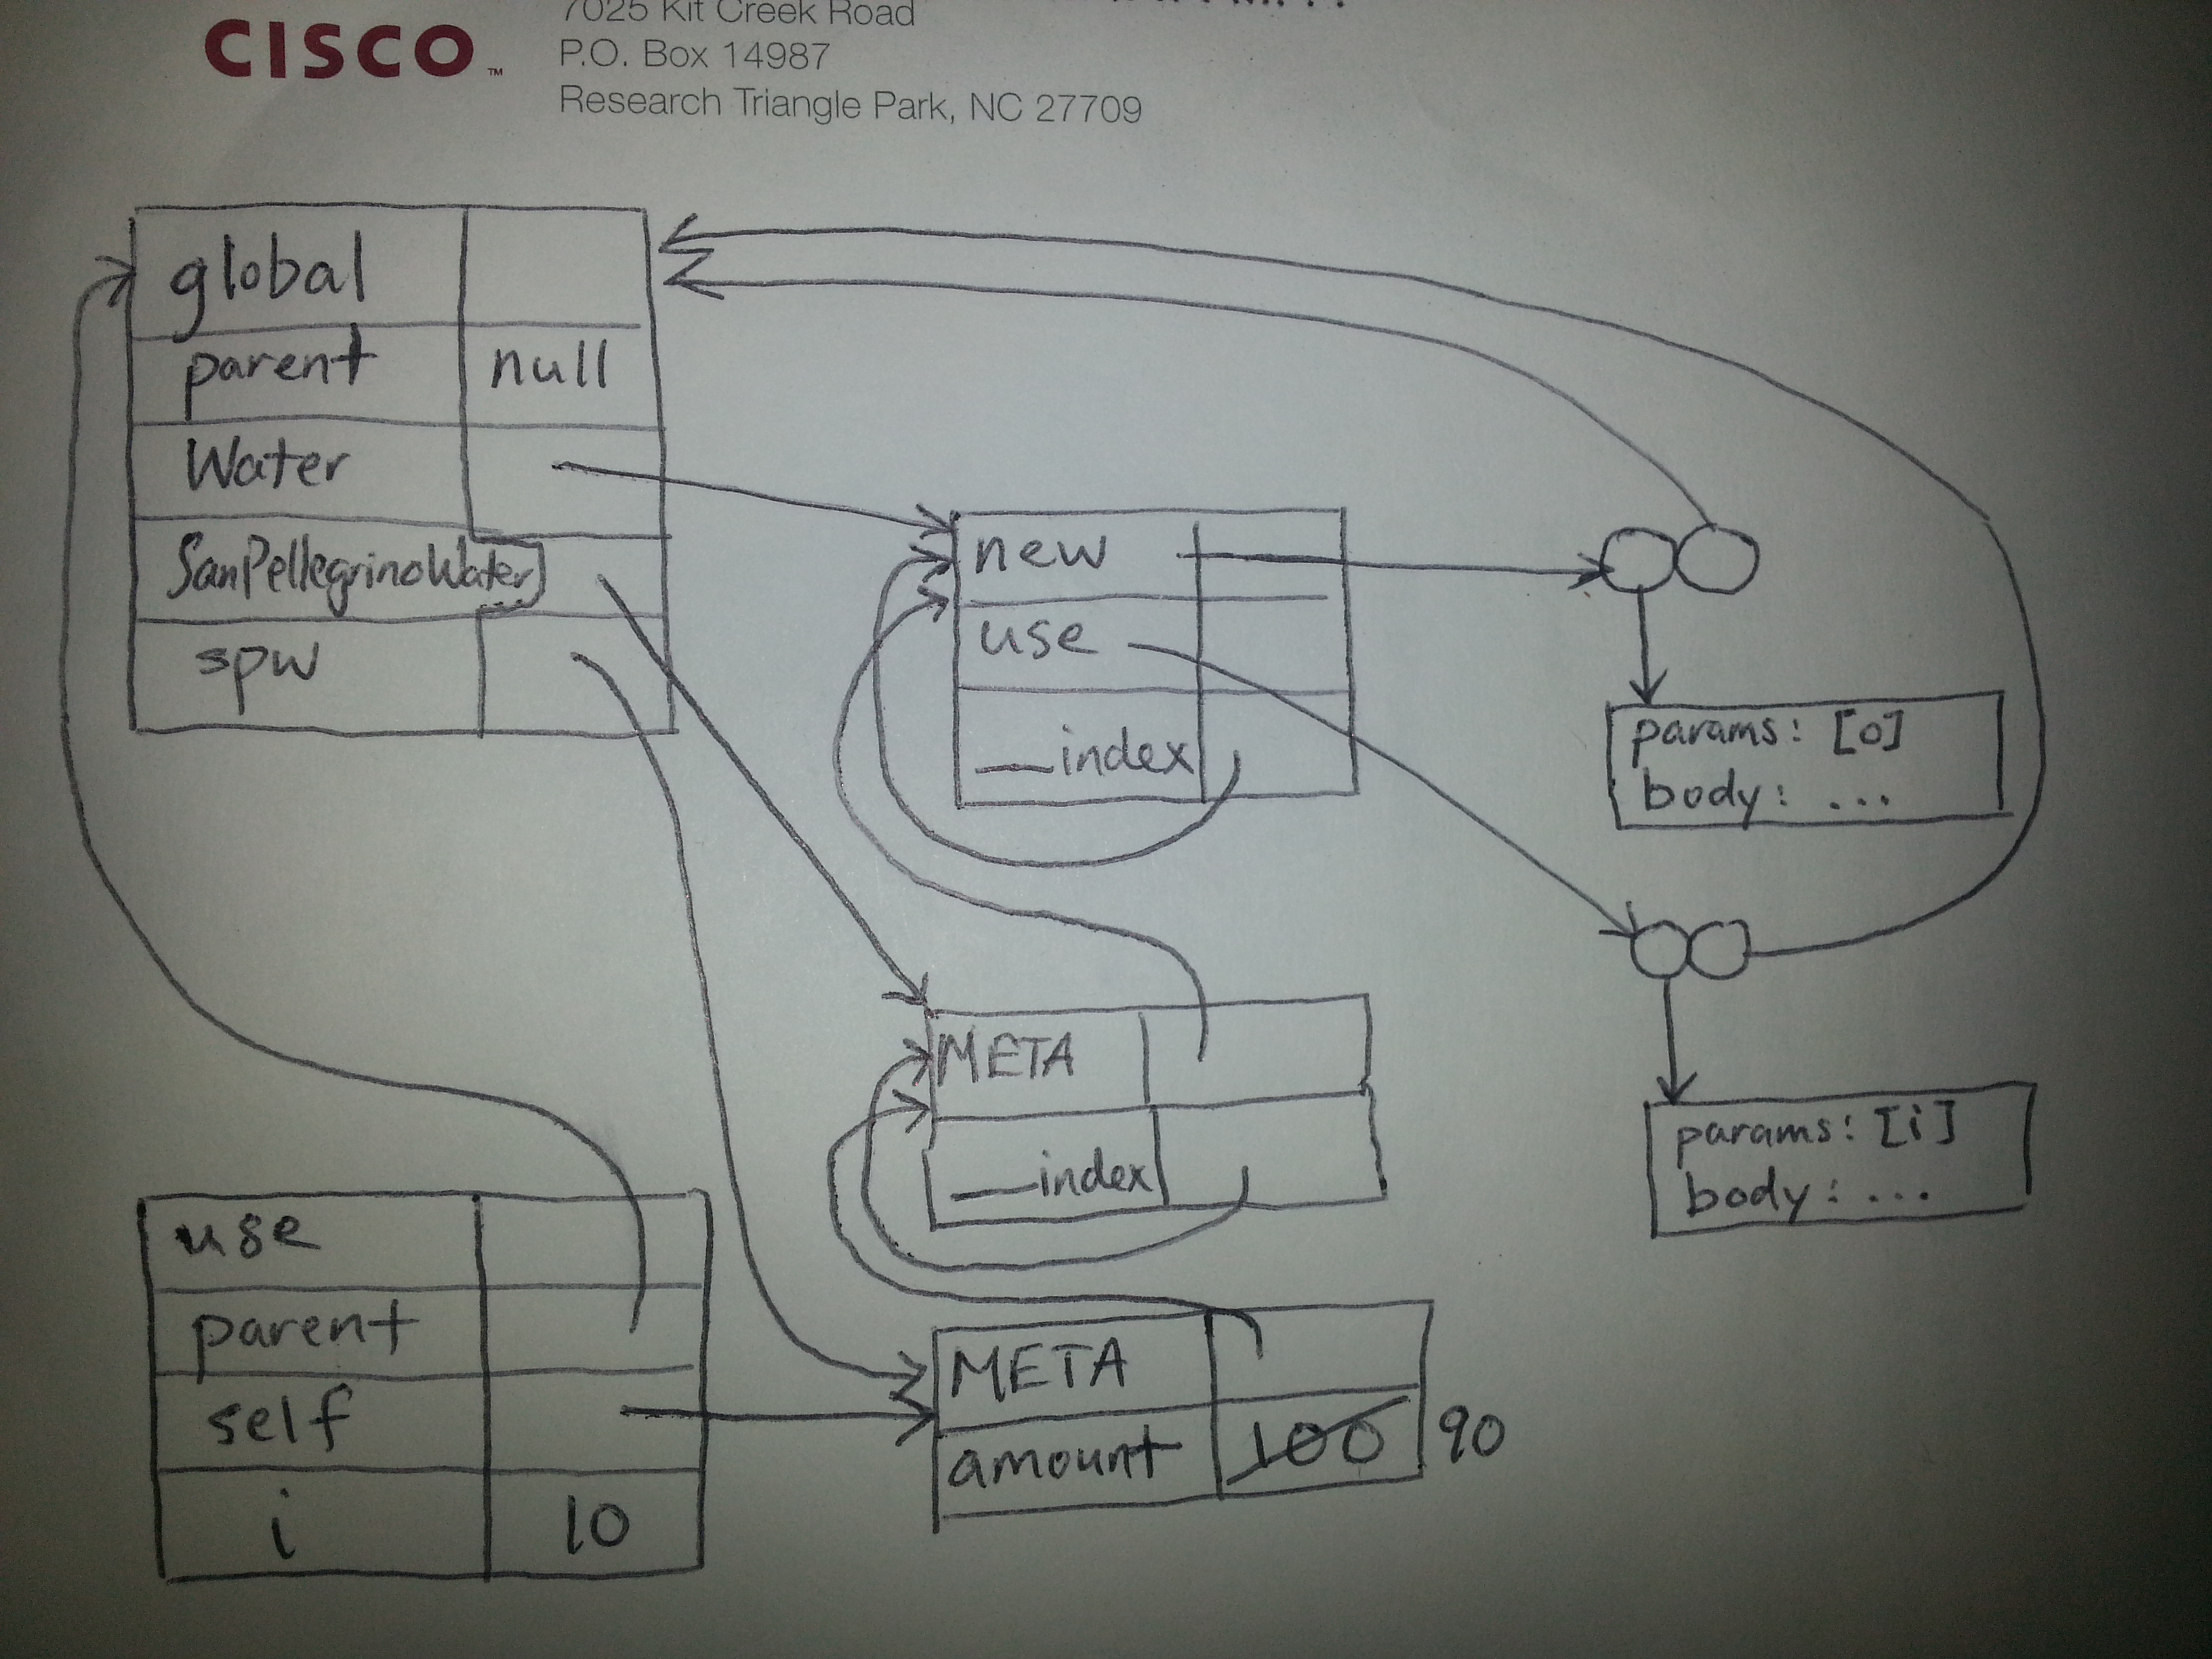
\includegraphics[scale=0.125]{env2}\\
Source line 26, called from line 31:\\
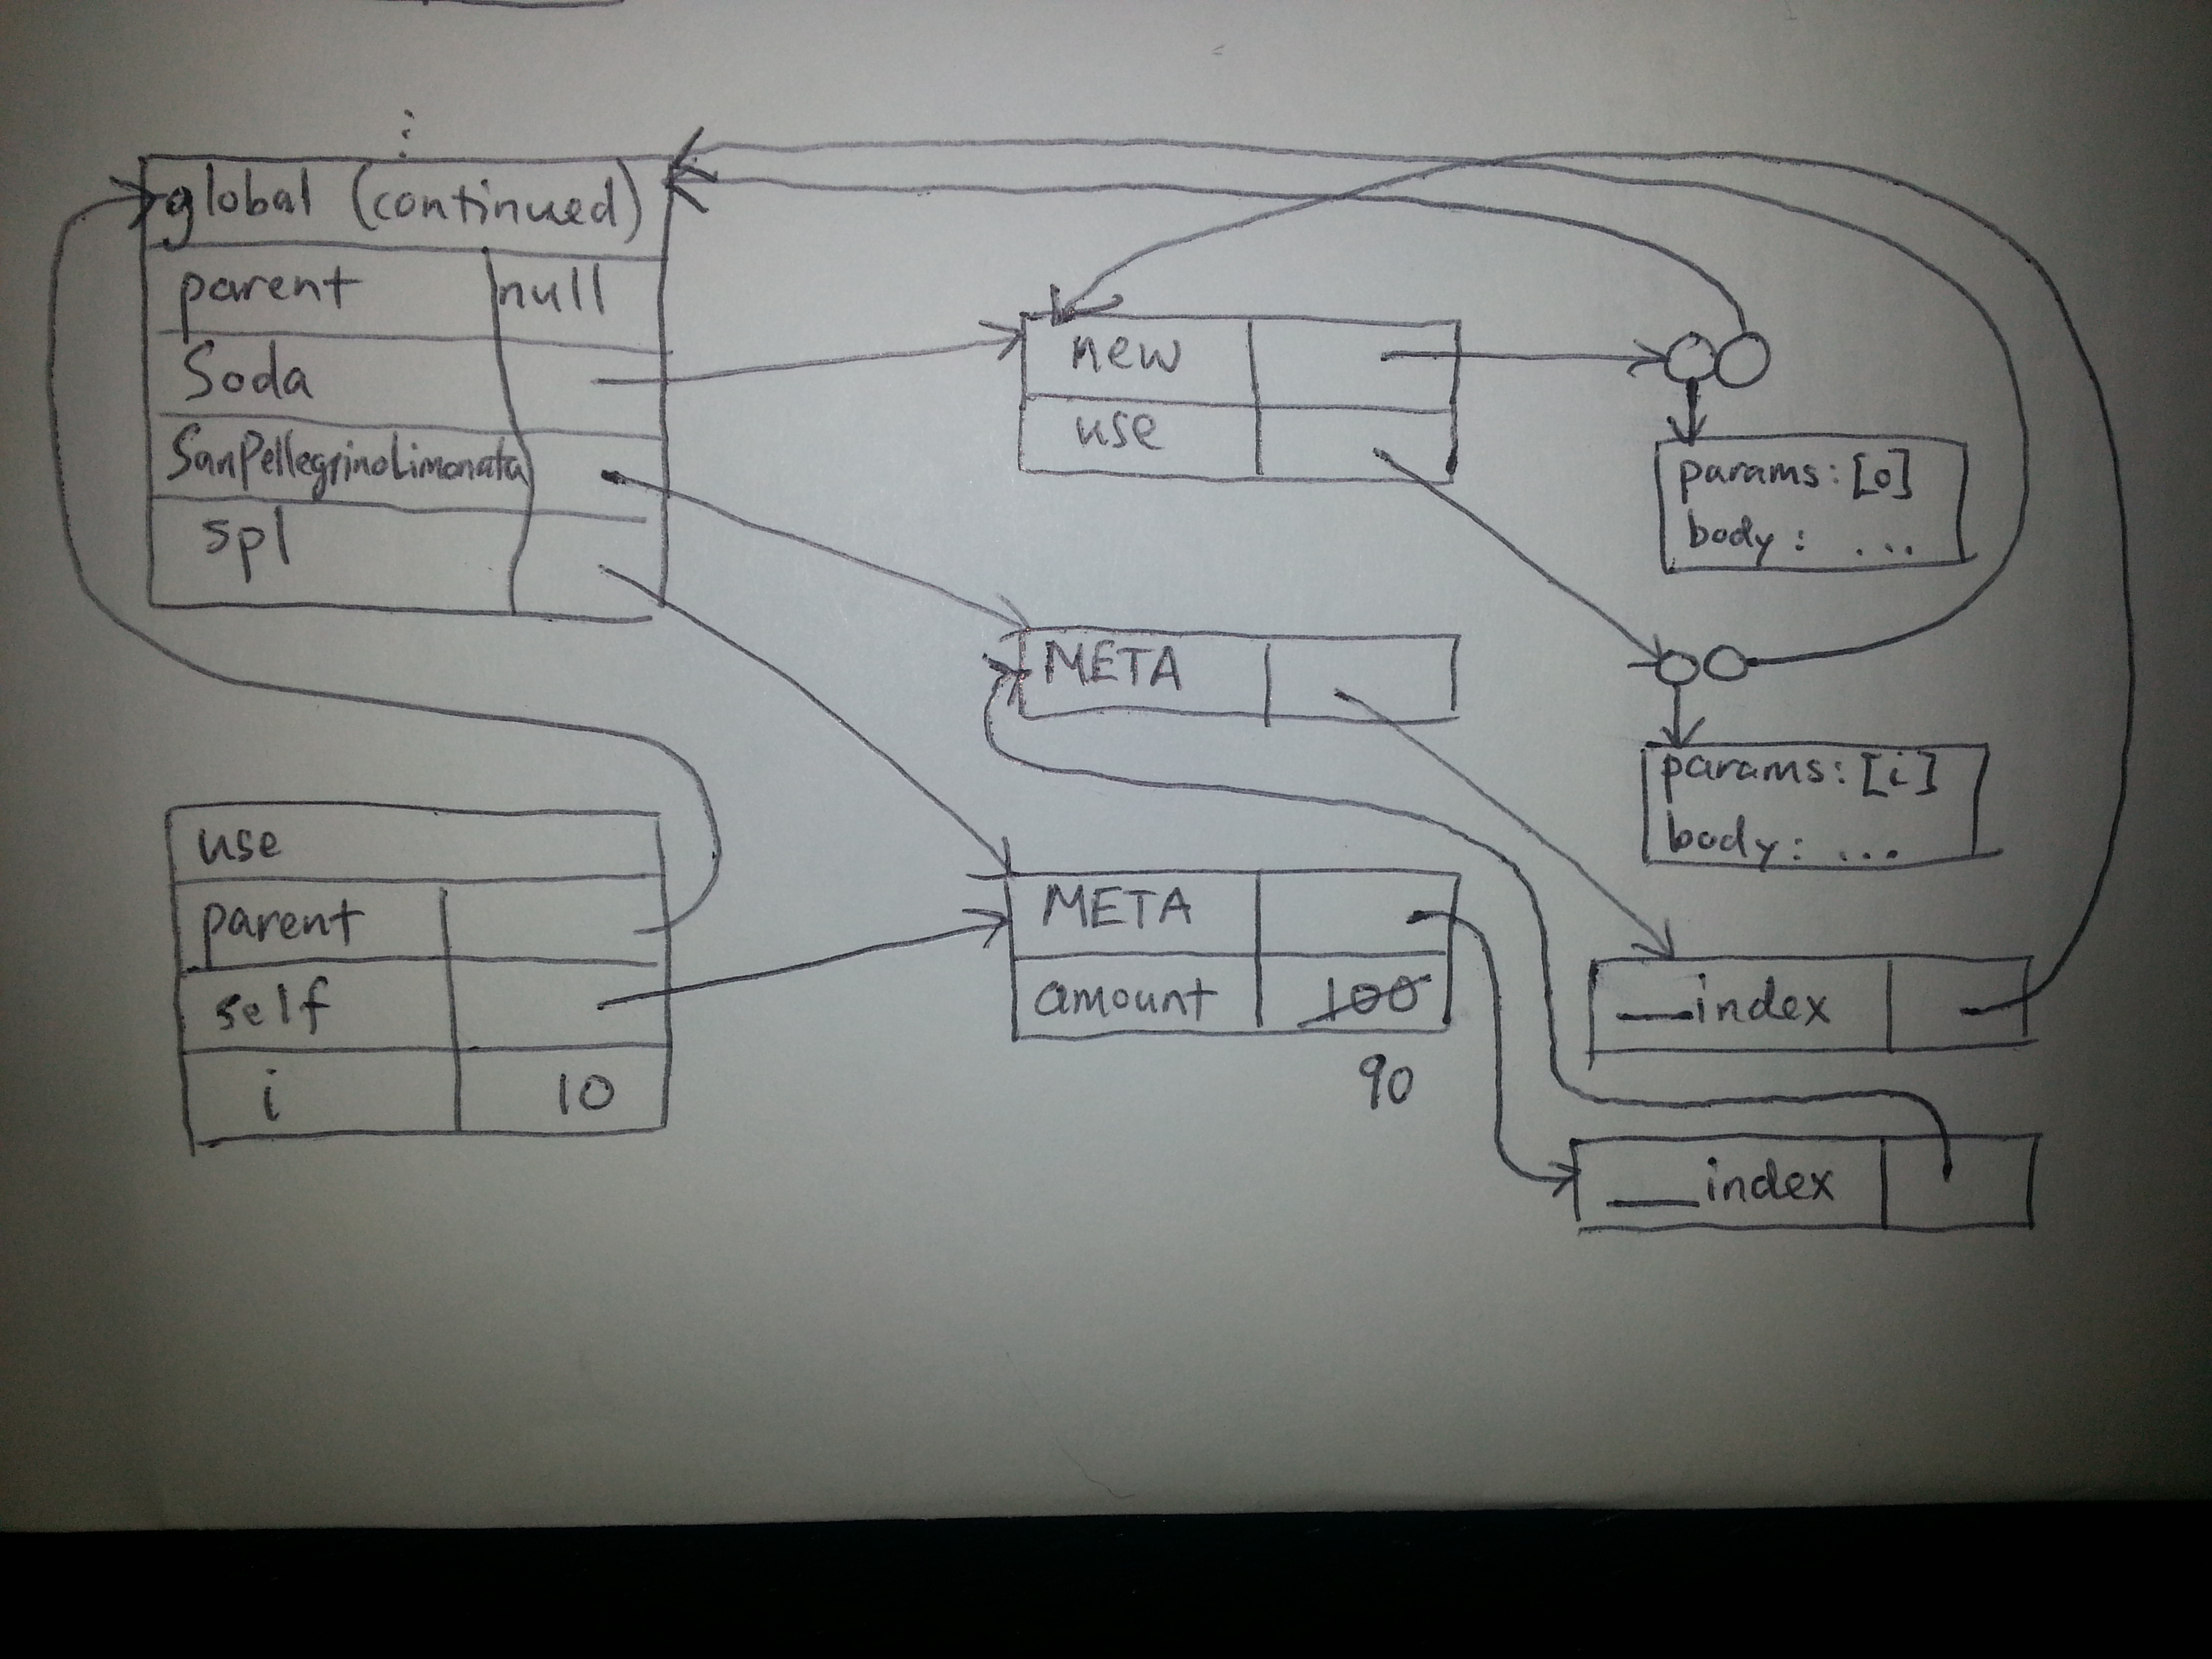
\includegraphics[scale=0.125]{env3}
\item For SanPellegrinoWater, the metatable is the Water object and its \texttt{\_\_index} field points to Water (itself). For SanPellegrinoLimonata, the metatable is a separate object whose \texttt{\_\_index} field points to Soda. This doesn't seem to affect the current inheritance hierarchy, as both halves of the code produce the expected results. Another level of inheritance wouldn't be affected in an unexpected way by either implementation because in both ways, the metatable of an object has an \texttt{\_\_index} field defined to refer to the proper supertype. It seems like metatables were introduced to specify methods for special behavior of objects, such as operator overloading, and \texttt{\_\_index} fields are the part of the metatable that looks up unresolved properties of an object.
\item Insert the following code after source line 13: \begin{verbatim}
SanPellegrinoWater.amount = 10000
\end{verbatim}
\newpage
\item Prototype-based inheritance allows us to create new types on the fly at runtime, instead of defining classes and outlining their blueprints beforehand. The lack of distinction between types and instances allows for easy modification of subtypes and supertypes at any time. \begin{verbatim}
SanPellegrinoWater = Water:new({})
...
spw = SanPellegrinoWater:new({})
SanPellegrinoWater.pH = 6.5
print(spw.pH) // prints 6.5
spw.pH = 6.0
print(spw.pH) // prints 6.0
print(SanPellegrinoWater.pH) // prints 6.5
\end{verbatim}
Class-based inheritance allows better organization of code to define each type. The separation of types and instances also provides a means of static type checking. \begin{verbatim}
class A:
    x = 2
    def __init__(self):
        self.y = 3
class B(A):
    def __init__(self):
        self.z = 4

# all type definitions go above this line

a = A()
b = B()
print(a.z) # static type checker could tell this won't work (if Python used one)
\end{verbatim}
\end{enumerate}


\newpage
\section*{Exercise 2}
\stepcounter{problemnumber}
\begin{enumerate}[(a)]
\item All \texttt{width} and \texttt{height} attributes are calculated from the bottom up, then all \texttt{x} and \texttt{y} attributes are calculated from the top down. \begin{verbatim}
HBox.children[i].y = HBox.y
HBox.height = max(HBox.children.map(lambda(c){c.height}))
VBox.children[i].x = VBox.x
VBox.children[i].y = VBox.y + sum(VBox.children[0 to i-1].map(lambda(c){c.height}))
VBox.width = max(VBox.children.map(lambda(c){c.width}))
VBox.height = sum(VBox.children.map(lambda(c){c.height}))
\end{verbatim}
\item We need 2 passes. The first goes from the bottom up to calculate the \texttt{width} and \texttt{height} of each node based on the same attributes of its children. Once we have these, we can fill in the \texttt{x} and \texttt{y} attributes of nodes from the top down until every leaf node has been assigned x and y values.
\item Pass \#1 - bottom up: \begin{verbatim}
HBox.width = sum(HBox.children.map(lambda(c){c.width}))
HBox.height = max(HBox.children.map(lambda(c){c.height}))
VBox.width = max(VBox.children.map(lambda(c){c.width}))
VBox.height = sum(VBox.children.map(lambda(c){c.height}))
\end{verbatim}
Pass \#2 - top down: \begin{verbatim}
HBox.children[i].x = HBox.x + sum(HBox.children[0 to i-1].map(lambda(c){c.width}))
HBox.children[i].y = HBox.y
VBox.children[i].x = VBox.x
VBox.children[i].y = VBox.y + sum(VBox.children[0 to i-1].map(lambda(c){c.height}))
\end{verbatim}
\end{enumerate}


\newpage
\section*{Exercise 3}
\stepcounter{problemnumber}
\begin{enumerate}[(a)]
\item There is a potential error on line 3 with the expression \texttt{x < 10}. If \texttt{x} is not of the integer type, this expression will produce an error. There is also a potential on line 4 with the expression \texttt{x(1)}. If execution of the code gets to this statement, then clearly \texttt{x} must have been an integer, which cannot be called. A third potential error is on line 8 with the expression \texttt{y * 4} because at this point \texttt{y} could be null and this expression wouldn't make sense.
\item \begin{verbatim}
function main(x: int): int {
  def y: int = 1
  if (x < 10) {
    x(1)
  } else {
    y = null
  }
  y * 4
}
\end{verbatim}
\item Type checking can prevent the error on line 3 by making sure \texttt{x} is an integer type. It can also prevent the error on line 4 by assinging \texttt{x} a type of \texttt{lambda(int) : int} but this would produce an error on line 3.
\item \begin{verbatim}
function main(x) {
  def y = 1
  if (x < 10) {
    x = lambda(x) {x}
    x(1)
    y * 4
  } else {
    null
  }
}
\end{verbatim}
\item Consider this snippet of code: \texttt{n: nonZeroInt = someFunction() - someOtherFunction()} In a realistic program, the results of the two function calls could produce the same \texttt{nonZeroInt} value such that the expression evaluates to zero. There's no way for a compiler to detect when this happens at compile time, so we'd end up with a runtime error of assigning the value 0 to a \texttt{nonZeroInt}, putting us back where we started.
\newpage
\item \begin{verbatim}
String[] a = new String[1];
Object[] b = a;
b[0] = new Integer(0);
char c = a[0].charAt(0);
\end{verbatim}
When the array is initialized with \texttt{new}, Java allocates memory specifically to hold objects of type \texttt{String} or any of its subtypes. At runtime, when we try to change the state of the array to hold an object of type \texttt{Integer}, Java catches that the dynamic type of the object to be stored doesn't fit with the static type of the array and throws an exception.
\end{enumerate}

\end{document}